% id: 19-08
% book: 베이직쎈 확률과 통계 · 01 여러 가지 순열
% section: 실전 감각 UP
% figure: tikz:fig-19-08
% answer: 
% answer_source: 
% variant_level: 0 (원본 전사)
% 이 파일은 build.mjs 가 items.json 에서 만든다. 고칠 때는 items.json 을 고친다.
\smash{\raisebox{1.5mm}{\dmkichul{베이직쎈 확률과 통계 19쪽 08번}}}
\noindent\begin{minipage}[t]{0.58\linewidth}\vspace{0pt}\raggedright 오른쪽 그림은 크기가 같은 정육면체 6개를 이어 붙여 만든 직육면체이다. 정육면체의 모서리를 따라 꼭짓점~$\pt{A}$에서 꼭짓점~$\pt{B}$까지 최단 거리로 가는 경우의 수는?\end{minipage}\hfill\begin{minipage}[t]{0.4\linewidth}\vspace{0pt}\centering \resizebox{\ifdim\width>\linewidth\linewidth\else\width\fi}{!}{% 19-08(19쪽) — 크기가 같은 정육면체 6개(가로 3 · 세로 2 · 높이 1)를 이어 붙인 직육면체와 꼭짓점 A, B.
% 스캔 화질이 낮아 TikZ 로 다시 그림(보이는 모서리 실선 · 숨은 모서리 파선 · 라벨은 원문에 있는 A, B 뿐 · 경우의 수는 적지 않는다).
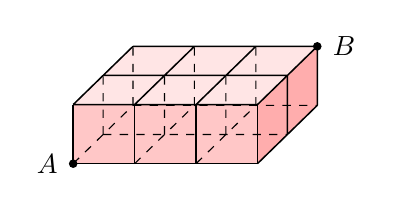
\begin{tikzpicture}[x={(0.78cm,0cm)},y={(0.38cm,0.37cm)},z={(0cm,0.75cm)},line width=0.55pt]
  \fill[red!10] (0,0,1) -- (3,0,1) -- (3,2,1) -- (0,2,1) -- cycle;
  \fill[red!22] (0,0,0) -- (3,0,0) -- (3,0,1) -- (0,0,1) -- cycle;
  \fill[red!32] (3,0,0) -- (3,2,0) -- (3,2,1) -- (3,0,1) -- cycle;
  % 숨은 모서리(아랫면 격자 · 왼쪽면 · 뒷면 · 속 모서리)
  \draw[dashed,line width=0.4pt] (0,0,0) -- (0,2,0) (1,0,0) -- (1,2,0) (2,0,0) -- (2,2,0)
    (0,1,0) -- (3,1,0) (0,2,0) -- (3,2,0)
    (0,1,0) -- (0,1,1) (0,2,0) -- (0,2,1) (1,1,0) -- (1,1,1) (1,2,0) -- (1,2,1)
    (2,1,0) -- (2,1,1) (2,2,0) -- (2,2,1);
  % 윗면 3x2 격자
  \draw (0,0,1) -- (3,0,1) (0,1,1) -- (3,1,1) (0,2,1) -- (3,2,1)
    (0,0,1) -- (0,2,1) (1,0,1) -- (1,2,1) (2,0,1) -- (2,2,1) (3,0,1) -- (3,2,1);
  % 앞면 3x1 · 오른쪽면 2x1
  \draw (0,0,0) -- (3,0,0) (0,0,0) -- (0,0,1) (1,0,0) -- (1,0,1) (2,0,0) -- (2,0,1) (3,0,0) -- (3,0,1);
  \draw (3,0,0) -- (3,2,0) (3,1,0) -- (3,1,1) (3,2,0) -- (3,2,1);
  \node[fill,circle,inner sep=1.1pt] at (0,0,0) {};
  \node[fill,circle,inner sep=1.1pt] at (3,2,1) {};
  \node[left=2pt] at (0,0,0) {$\pt{A}$};
  \node[right=2pt] at (3,2,1) {$\pt{B}$};
\end{tikzpicture}
}\end{minipage}\par
\dmchoicesauto{}{$52$}{$56$}{$60$}{$64$}{$68$}
